\documentclass[a4paper, 10pt]{article}
\usepackage{trymtex}


\title{Numerical Solution of Differential Equations\\by Difference Methods}
\author{Trym Sæther}
\date{\today}
\begin{document}

\sloppy

\maketitle
\tableofcontents
\newpage

\section{Endelig differansemetoder (FDM)}

FDM er en numerisk metode for å løse ODE og PDE ved å diskretisere domenet og tilnærme den deriverte med differanser.

\subsection*{Motivasjon}

Gitt en vilkårlig differensiallikning (ODE), som f.eks. \( \ddn[2]{f(x)}{x} = f(x) - x^3 \)\label{eq:ode} med randbetingelser: \( f(x_0) = \alpha \) og \( f(x_N) = \beta \).
Denne ODE har allerede en eksakt løsning: \( f(x) = c_0e^x + c_1e^{-x} + x^3 + 6x \)\label{eq:exact}.
Men, hva om vi ikke har en eksakt løsning? Da kan vi bruke FDM til å tilnærme løsningen.

\subsection*{FDM-oppskrift}

\begin{enumerate}
    \item \textbf{Diskretisering:} Del intervallet \(x \in [\alpha, \beta]\) inn i \(N\) like store delintervaller med \(x_i = \alpha + ih\) for \(i = 0,1,\ldots,N\) og \(h = 2/N\)
    \item \textbf{Taylor-utvikling:} Rekkeutvikle \(f(x \pm h)\) rundt \(x\).
    \item \textbf{Differanse metoder:} Finn en lineærkombinasjon av \(f(x \pm h)\) som tilnærmer den deriverte.
          \begin{align}
              C_{-1}f(x - h) + C_0f(x) + C_1f(x + h)   & = \dd[2]{f(x)}{x} + \mathcolor{blue}{O(h)} \tag{Sentrum} \label{eq:center}     \\
              C_{0}f(x) + C_1f(x + h ) + C_2f(x + 2h)  & = \dd[2]{f(x)}{x} + \mathcolor{blue}{O(h^2)} \tag{Fremover} \label{eq:forward} \\
              C_{-2}f(x - 2h) + C_{-1}f(x-h) + C_0f(x) & = \dd[2]{f(x)}{x} + \mathcolor{blue}{O(h)} \tag{Bakover} \label{eq:backward}
          \end{align}
    \item \textbf{Diskretiser og løs ODE:} Anvend en av disse metodene, f.eks. \ref{eq:center} på \ref{eq:ode} og løs ligningssettet \(T_h \vec{f} = \vec{b}\), hvor \(T_h\) er en tri-diagonal.
\end{enumerate}

\subsection{Differanseoperatorer}
\begin{definition}{Differanseoperatorer}{}
    \begin{align*}
        \delta_h u(x) = u(x + h/2) - u(x - h/2) \tag{Sentral differanseoperator} \label{eq:central_diff}                           \\
        \mu_h u(x) = \frac{1}{2} \left( u(x + h/2) + u(x - h/2) \right) \tag{Gjennomsnittsoperator} \label{eq:avg_op}              \\
        \Delta_h u(x) = u(x + h) - u(x) \tag{Fremover differanseoperator} \label{eq:forward_diff}                                  \\
        \nabla_h u(x) = u(x) - u(x - h) \tag{Bakover differanseoperator} \label{eq:backward_diff}                                  \\
        \delta_h^2 u(x) = u(x + h) - 2u(x) + u(x - h) \tag{Andre ordens sentral differanseoperator} \label{eq:second_central_diff} \\
        E_h u(x) = u(x + h) \tag{Flytt operator} \label{eq:shift_op}                                                               \\
    \end{align*}
\end{definition}


\subsection*{Stenciler}

\begin{figure}[ht]
    \centering
    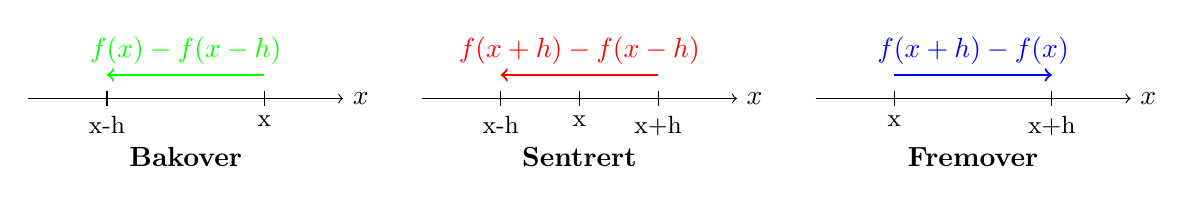
\begin{tikzpicture}
        % Backward Difference Scope
            \begin{scope}[xshift=-5cm]
                \draw[->] (-1,0) -- (3,0) node[right] {$x$}; % Number Line
                \foreach \x/\label in {0/$x-h$, 2/$x$} {
                \draw (\x,0.1) -- (\x,-0.1); % Points
                \node[below] at (\x,-0.1) {\small $\label$}; % Labels
                }
                \draw[->, thick, green] (2,0.3) -- (0,0.3) node[midway, above] {$f(x) - f(x-h)$}; % Arrow for difference
                \node[below] at (1, -0.5) {\textbf{Bakover}}; % Label
            \end{scope}
            
            % Central Difference Scope
            \begin{scope}[xshift=0cm]
                \draw[->] (-1,0) -- (3,0) node[right] {$x$};
                \foreach \x/\label in {0/$x-h$, 1/$x$, 2/$x+h$} {
                \draw (\x,0.1) -- (\x,-0.1); % Points
                \node[below] at (\x,-0.1) {\small $\label$}; 
                }
                \draw[->, thick, red] (2,0.3) -- (0,0.3) node[midway, above] {$f(x+h) - f(x-h)$};
                \node[below] at (1, -0.5) {\textbf{Sentrert}};
            \end{scope}
            
            % Forward Difference Scope
            \begin{scope}[xshift=5cm]
                \draw[->] (-1,0) -- (3,0) node[right] {$x$};
                \foreach \x/\label in {0/$x$, 2/$x+h$} {
                \draw (\x,0.1) -- (\x,-0.1);
                \node[below] at (\x,-0.1) {\small $\label$};
                }
                \draw[->, thick, blue] (0,0.3) -- (2,0.3) node[midway, above] {$f(x+h) - f(x)$};
                \node[below] at (1, -0.5) {\textbf{Fremover}};
            \end{scope}
    \end{tikzpicture}
    \caption{Finite Difference Stencils: Backward, Central, and Forward Difference}
    \label{fig:finite-differences}
\end{figure}


Som figuren viser, benytter \textbf{fremover}-differanser hovedsakelig punkter \emph{til høyre} for \(x_i\),
\textbf{bakover}-differanser benytter hovedsakelig punkter \emph{til venstre} for \(x_i\),
mens \textbf{sentrerte}-differanser er symmetriske rundt \(x_i\).


\section*{Endelig differanseskjema}

Endelige differanseformler gir diskrete tilnærminger av deriverte ved å bruke funksjonsverdier i strategisk utvalgte punkter (ofte kalt \emph{stencil}).
Kolonnene merket \(\mathbf{-3}\) til \(\mathbf{+3}\) (eller flere, avhengig av formelens bredde) oppgir \emph{dimensjonsløse koeffisienter} som multipliserer funksjonsverdiene i \(x_{i + k}\).

For å beregne den deriverte numerisk, må du så dividere med \(h^n\), der \(n\) er den deriverteordenen:

\[
    \frac{d^n f}{dx^n} \Bigg|_{x_i} \approx \frac{1}{h^n} \sum_{k=-m}^{m} \bigl( c_k f(x_{i+k}) \bigr)
\]

\begin{itemize}
    \item \(m\) er halvparten av stencilens bredde (f.eks. 3 for en 7-punkts stencil).
    \item \(c_k\) er dimensjonsløse koeffisienter.
\end{itemize}
\begin{example}{4 deriverte med framoverdifferanser}{}
    For å tilnærme den fjerde deriverte av en funksjon \(f(x)\) med en 7-punkts fremoverdifferanse, bruker vi formelen:

    \[
        \frac{d^4 f}{dx^4} \Bigg|_{x_i} \approx \frac{1}{h^4} \left( c_{-3} f(x_{i-3}) + c_{-2} f(x_{i-2}) + c_{-1} f(x_{i-1}) + c_0 f(x_i) + c_1 f(x_{i+1}) + c_2 f(x_{i+2}) + c_3 f(x_{i+3}) \right)
    \]

    Koeffisientene for en 7-punkts fremoverdifferanse er gitt i tabellen.
\end{example}

\begin{table}[H]
    \centering
    \setlength{\tabcolsep}{5pt}
    \renewcommand{\arraystretch}{1.2}
    \begin{tabular}{|c|c|c|c|c|c|c|c|c|c|}
        \hline
        \rowcolor{cyan!20} \textbf{\footnotesize{Metode}} & \textbf{\footnotesize{Der.}} & \textbf{\footnotesize Acc.} & $\mathbf{-3}$    & $\mathbf{-2}$    & $\mathbf{-1}$   & $\mathbf{0}$     & $\mathbf{1}$      & $\mathbf{2}$       & $\mathbf{3}$     \\ \hline

        \multirow{12}{*}{\textbf{\footnotesize{Forover}}}
                                                          & \multirow{3}{*}{1}           & 2                           &                  &                  & $-1$            & $1$              &                   &                    &                  \\ \cline{3-10}
                                                          &                              & 4                           &                  & $\frac{1}{6}$    & $-\frac{2}{3}$  & $1$              &                   &                    &                  \\ \cline{3-10}
                                                          &                              & 6                           & $-\frac{1}{60}$  & $\frac{3}{20}$   & $-\frac{3}{4}$  & $1$              &                   &                    &                  \\ \cline{2-10}
                                                          & \multirow{3}{*}{2}           & 2                           &                  &                  & $1$             & $-2$             & $1$               &                    &                  \\ \cline{3-10}
                                                          &                              & 4                           &                  & $-\frac{1}{12}$  & $\frac{4}{3}$   & $-\frac{5}{2}$   & $\frac{4}{3}$     & $-\frac{1}{12}$    &                  \\ \cline{3-10}
                                                          &                              & 6                           & $\frac{1}{90}$   & $-\frac{3}{20}$  & $\frac{3}{2}$   & $-\frac{49}{18}$ & $\frac{3}{2}$     & $-\frac{3}{20}$    &                  \\ \cline{2-10}
                                                          & \multirow{3}{*}{3}           & 2                           &                  &                  & $-1$            & $3$              & $-3$              & $1$                &                  \\ \cline{3-10}
                                                          &                              & 4                           &                  & $\frac{1}{8}$    & $-1$            & $\frac{13}{8}$   & $-1$              & $\frac{1}{8}$      &                  \\ \cline{3-10}
                                                          &                              & 6                           & $-\frac{1}{120}$ & $\frac{1}{8}$    & $-1$            & $\frac{13}{8}$   & $-1$              & $\frac{1}{8}$      & $-\frac{1}{120}$ \\ \cline{2-10}
                                                          & \multirow{3}{*}{4}           & 2                           &                  &                  & $1$             & $-4$             & $6$               & $-4$               & $1$              \\ \cline{3-10}
                                                          &                              & 4                           &                  & $-\frac{1}{6}$   & $2$             & $-\frac{13}{2}$  & $\frac{28}{3}$    & $-\frac{13}{2}$    & $2$              \\ \cline{3-10}
                                                          &                              & 6                           & $\frac{1}{180}$  & $-\frac{2}{9}$   & $\frac{19}{18}$ & $-\frac{65}{18}$ & $\frac{916}{180}$ & $-\frac{65}{18}$   & $\frac{19}{18}$  \\ \hline

        \multirow{12}{*}{\textbf{\footnotesize{Sentrert}}}
                                                          & \multirow{3}{*}{1}           & 2                           &                  & $-\frac{1}{2}$   &                 & $\frac{1}{2}$    &                   &                    &                  \\ \cline{3-10}
                                                          &                              & 4                           & $\frac{1}{12}$   & $-\frac{2}{3}$   &                 & $\frac{2}{3}$    & $-\frac{1}{12}$   &                    &                  \\ \cline{3-10}
                                                          &                              & 6                           & $-\frac{1}{60}$  & $\frac{3}{20}$   & $-\frac{3}{4}$  &                  & $\frac{3}{4}$     & $-\frac{3}{20}$    & $\frac{1}{60}$   \\ \cline{2-10}
                                                          & \multirow{3}{*}{2}           & 2                           &                  & $\frac{1}{2}$    & $-1$            & $0$              & $1$               & $-\frac{1}{2}$     &                  \\ \cline{3-10}
                                                          &                              & 4                           &                  & $-\frac{1}{12}$  & $\frac{4}{3}$   & $-\frac{5}{2}$   & $\frac{4}{3}$     & $-\frac{1}{12}$    &                  \\ \cline{3-10}
                                                          &                              & 6                           & $-\frac{1}{90}$  & $\frac{3}{20}$   & $-\frac{3}{2}$  & $\frac{49}{18}$  & $-\frac{3}{2}$    & $\frac{3}{20}$     & $\frac{1}{90}$   \\ \cline{2-10}
                                                          & \multirow{3}{*}{3}           & 2                           &                  & $-\frac{1}{2}$   & $1$             & $0$              & $-1$              & $\frac{1}{2}$      &                  \\ \cline{3-10}
                                                          &                              & 4                           &                  & $\frac{1}{8}$    & $-1$            & $\frac{13}{8}$   & $-1$              & $\frac{1}{8}$      &                  \\ \cline{3-10}
                                                          &                              & 6                           & $\frac{1}{90}$   & $-\frac{3}{20}$  & $\frac{3}{2}$   & $-\frac{13}{8}$  & $1$               & $\frac{3}{20}$     & $-\frac{1}{90}$  \\ \cline{2-10}
                                                          & \multirow{3}{*}{4}           & 2                           &                  & $1$              & $-4$            & $6$              & $-4$              & $1$                &                  \\ \cline{3-10}
                                                          &                              & 4                           &                  & $-\frac{1}{6}$   & $2$             & $-\frac{13}{2}$  & $\frac{28}{3}$    & $-\frac{13}{2}$    & $2$              \\ \cline{3-10}
                                                          &                              & 6                           & $\frac{1}{180}$  & $-\frac{2}{9}$   & $\frac{19}{18}$ & $-\frac{65}{18}$ & $\frac{916}{180}$ & $-\frac{65}{18}$   & $\frac{19}{18}$  \\ \hline

        \multirow{12}{*}{\textbf{\footnotesize{Bakover}}}
                                                          & \multirow{3}{*}{1}           & 2                           &                  & $1$              & $-1$            &                  &                   &                    &                  \\ \cline{3-10}
                                                          &                              & 4                           &                  & $-\frac{1}{6}$   & $\frac{2}{3}$   & $-1$             &                   &                    &                  \\ \cline{3-10}
                                                          &                              & 6                           & $\frac{1}{60}$   & $-\frac{3}{20}$  & $\frac{3}{4}$   & $-1$             &                   &                    &                  \\ \cline{2-10}
                                                          & \multirow{3}{*}{2}           & 2                           &                  & $-1$             & $2$             & $-1$             &                   &                    &                  \\ \cline{3-10}
                                                          &                              & 4                           &                  & $\frac{1}{12}$   & $-\frac{4}{3}$  & $\frac{5}{2}$    & $-\frac{4}{3}$    & $\frac{1}{12}$     &                  \\ \cline{3-10}
                                                          &                              & 6                           & $-\frac{1}{90}$  & $\frac{3}{20}$   & $-\frac{3}{2}$  & $\frac{49}{18}$  & $-\frac{3}{2}$    & $\frac{3}{20}$     & $-\frac{1}{90}$  \\ \cline{2-10}
                                                          & \multirow{3}{*}{3}           & 2                           &                  & $1$              & $-3$            & $3$              & $-1$              &                    &                  \\ \cline{3-10}
                                                          &                              & 4                           &                  & $-\frac{1}{8}$   & $1$             & $-\frac{13}{8}$  & $1$               & $\frac{1}{8}$      &                  \\ \cline{3-10}
                                                          &                              & 6                           & $\frac{1}{90}$   & $-\frac{3}{20}$  & $\frac{3}{2}$   & $-\frac{13}{8}$  & $1$               & $\frac{3}{20}$     & $-\frac{1}{90}$  \\ \cline{2-10}
                                                          & \multirow{3}{*}{4}           & 2                           &                  & $-1$             & $4$             & $-6$             & $4$               & $-1$               &                  \\ \cline{3-10}
                                                          &                              & 4                           &                  & $\frac{1}{6}$    & $-2$            & $\frac{13}{2}$   & $-\frac{28}{3}$   & $\frac{13}{2}$     & $-2$             \\ \cline{3-10}
                                                          &                              & 6                           &                  & $-\frac{1}{180}$ & $\frac{2}{9}$   & $-\frac{19}{18}$ & $\frac{65}{18}$   & $-\frac{916}{180}$ & $\frac{65}{18}$  \\ \hline
    \end{tabular}
    \caption{Koeffisienter for endelige differanser for deriverte opptil fjerde orden.
        Kolonnene \(\mathbf{-3}\) til \(\mathbf{+3}\) (eller mer) viser de dimensjonsløse koeffisientene i front av \(f(x_{i+k})\).
        Til slutt divideres sumproduktet med \(h^n\) for en \(n\)-te deriverte.
        «Acc.» angir den formelle nøyaktighetsordenen.}
    \label{tab:finite_difference_table}
\end{table}

\vspace{1em}

\noindent\textbf{Tips for bruk:}
\begin{itemize}
    \item Kontroller alltid \emph{tegnkonvensjon og indeksering}:
          \(\;f(x_{i+k}) \leftrightarrow \text{koeffisient under kolonne }k\).
    \item Etter at koeffisientene er multiplisert med funksjonsverdiene, \emph{divider med} \(h^n\) for en \(n\)-te deriverte.
    \item Fremover/bakover-stenciler brukes ofte nær kantene av et domene for å unngå ute-av-rekkevidde-punkter.
    \item Sentrerte differanser gir vanligvis mindre feilkonstanter i indre punkter, men krever funksjonsverdier på begge sider av \(x_i\).
\end{itemize}




\subsubsection{Bakover differanseoperator}
\begin{align*}
    \nabla_h u_m & = u_m - u_{m-1}                                                                                                                            \\
                 & = u_m - \left[u_m - h u_m^{\prime} + \frac{h^2}{2} u_m^{\prime\prime} - \frac{h^3}{6} u_m^{(3)} + \frac{h^4}{24} u_m^{(4)} - \hdots\right] \\
                 & = h u_m^{\prime} - \frac{h^2}{2} u_m^{\prime\prime} + \frac{h^3}{6} u_m^{(3)} - \frac{h^4}{24} u_m^{(4)} + \hdots                          \\
                 & = h u_m^{\prime} + O(h^2)                                                                                                                  \\
                 & = O(h)
\end{align*}

\begin{align*}
    \nabla_h^2 u_m & = u_m - 2u_{m-1} + u_{m-2}                                                                                                                   \\
                   & = u_m                                                                                                                                        \\
    - 2            & \left[u_m - h u_m^{\prime} + \frac{h^2}{2} u_m^{\prime\prime} - \frac{h^3}{6} u_m^{(3)} + \frac{h^4}{24} u_m^{(4)} - \hdots\right]           \\
    +              & \left[u_m - 2h u_m^{\prime} + \frac{4h^2}{2} u_m^{\prime\prime} - \frac{8h^3}{6} u_m^{(3)} + \frac{16h^4}{24} u_m^{(4)} - \hdots\right]      \\
                   & = h^2 u_m^{\prime\prime} - 2h^2 u_m^{\prime\prime} + \frac{2h^3}{3} u_m^{(3)} - \frac{4h^3}{3} u_m^{(3)} + \frac{4h^4}{3} u_m^{(4)} - \hdots \\
                   & = h^2 u_m^{\prime\prime} - h^3 u_m^{(3)} + \frac{7h^4}{12} u_m^{(4)} + O(h^5)                                                                \\
                   & = h^2 u_m^{\prime\prime} - h^3 u_m^{(3)} + O(h^4)                                                                                            \\
                   & = O(h^2)
\end{align*}

\begin{align*}
    \nabla_h^3 u_m & = u_m - 3u_{m-1} + 3u_{m-2} - u_{m-3}                                                                                                    \\
                   & = u_m                                                                                                                                    \\
    - 3            & \left[u_m - h u_m^{\prime} + \frac{h^2}{2} u_m^{\prime\prime} - \frac{h^3}{6} u_m^{(3)} + \frac{h^4}{24} u_m^{(4)} - \hdots\right]       \\
    + 3            & \left[u_m - 2h u_m^{\prime} + \frac{4h^2}{2} u_m^{\prime\prime} - \frac{8h^3}{6} u_m^{(3)} + \frac{16h^4}{24} u_m^{(4)} - \hdots\right]  \\
    -              & \left[u_m - 3h u_m^{\prime} + \frac{9h^2}{2} u_m^{\prime\prime} - \frac{27h^3}{6} u_m^{(3)} + \frac{81h^4}{24} u_m^{(4)} - \hdots\right] \\
                   & = h^3 u_m^{(3)} - 3h^3 u_m^{(3)} + \frac{3h^4}{2} u_m^{(4)} - \frac{9h^4}{2} u_m^{(4)} + \hdots                                          \\
                   & = h^3 u_m^{(3)} - \frac{3h^4}{2} u_m^{(4)} + O(h^5)                                                                                      \\
                   & = h^3 u_m^{(3)} + O(h^4)                                                                                                                 \\
                   & = O(h^3)
\end{align*}

\begin{example}{}{}
    \( f''(x) = f(x) - x^3 \) med \( [f(0), f(2)] = [0, 20] \) og \( N = 5 \). Det gir 1D FDM-ligningssettet med sentral differanseoperator:
    \begin{align*}
        \overbrace{
            \begin{bmatrix}
                1             & 0                  & 0             & \cdots & 0             \\
                \frac{1}{h^2} & -\frac{2}{h^2} - 1 & \frac{1}{h^2} & \cdots & 0             \\
                0             & \ddots             & \ddots        & \ddots & \vdots        \\
                \vdots        & \ddots             & \ddots        & \ddots & \frac{1}{h^2} \\
                0             & \cdots             & 0             & 0      & 1
            \end{bmatrix}}^{L_h}
        \overbrace{
            \begin{bmatrix}
                f(x_0) \\ f(x_1) \\ \vdots \\ f(x_{N-1}) \\ f(x_N)
            \end{bmatrix}}^{\vec{f}}
                    & =
        \overbrace{
        \begin{bmatrix}
                \alpha \\ h^2(x_1^3 - x_1) \\ \vdots \\ h^2(x_{N-1}^3 - x_{N-1}) \\ \beta
            \end{bmatrix}}^{\vec{b}} \\
        L_h \vec{f} & = \vec{b}\tag{SUS!}
    \end{align*}

    \vspace{0.5em}

    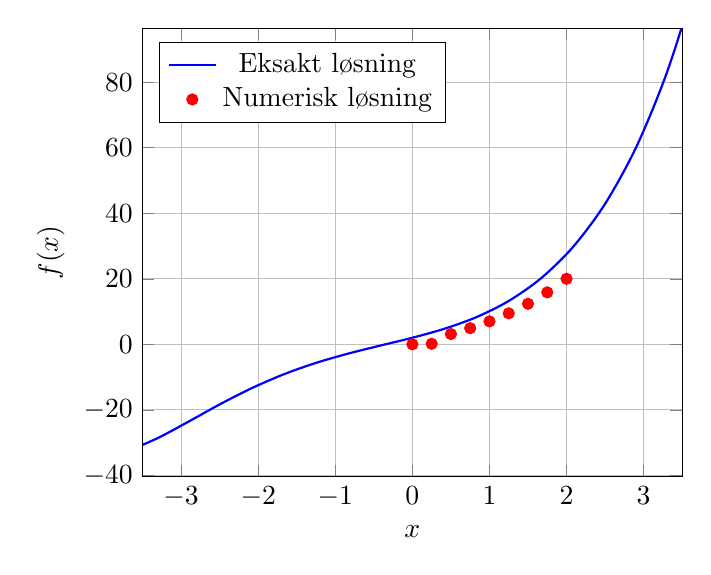
\begin{tikzpicture}
        \begin{axis}[
                xlabel={\(x\)},
                ylabel={\(f(x)\)},
                grid=major,
                legend pos=north west,
                xmin=-3.5,
                xmax=3.5,
                xtick={-3, -2, -1, 0, 1, 2, 3},
            ]
            \addplot[smooth, thick, blue] {x^3 + 6*x + exp(x) + exp(-x)};
            \addplot[only marks, red] coordinates {
                    (0, 0)
                    (0.25, 0.1516)
                    (0.5, 3.125)
                    (0.75, 4.922)
                    (1, 7)
                    (1.25, 9.453)
                    (1.5, 12.375)
                    (1.75, 15.859)
                    (2, 20)
                };
            \legend{Eksakt løsning, Numerisk løsning}
        \end{axis}
    \end{tikzpicture}
    \label{fig:ode}
\end{example}
\chapter{\gls{fem}}
\glsdesc{fem}

\begin{equation}
  u(x) \approx \sum_{i=1}^N c_i \phi_i(x)
\end{equation}

\paragraph{Betingelser}

For å bruke \gls{fem} til å løse et \gls{pde}-problem, må problemet oppfylle følgende betingelser:

\begin{itemize}
  \item \textbf{Linearitet:} Problemet må være lineært, dvs. ligningene kan uttrykkes som \(\mathcal{L}(u) = f\), hvor \(\mathcal{L}\) er en lineær operator.
  \item \textbf{Kontinuerlig Differensierbar:} Løsningen \( u(x) \) må være kontinuerlig differensierbar i \gls{domain}et \( \Omega \).
  \item \textbf{Geometrisk Enkelhet:} \gls{domain}et \( \Omega \) bør kunne deles opp i enkle geometriske elementer (f.eks. trekanter, firkanter i 2D, tetraedre i 3D):
        \[
          \Omega = \bigcup_{e=1}^{E} \Omega_e
        \]
  \item \textbf{Kvantiserbarhet:} Problemet må være kvantiserbart, dvs. løsningen kan tilnærmes godt ved hjelp av en endelig \gls{basisfunction}:
        \[
          u_h(x) = \sum_{i=1}^{N} c_i \phi_i(x)
        \]
  \item \textbf{Randbetingelser:} Randbetingelsene må være kompatible med valg av funksjonsrom:
        \[
          u|_{\partial \Omega} = g \quad \text{eller} \quad \frac{\partial u}{\partial n}\bigg|_{\partial \Omega} = h
        \]
\end{itemize}

\section{Oppskrift}

\begin{enumerate}
  \item \textbf{\gls{discretization}:} Del \gls{domain}et \( \Omega \) inn i enkle geometriske elementer \( \Omega_e \) og tilnærme løsningen med en lineærkombinasjon av \gls{basisfunction}er:
        \[
          u(x) \approx \sum_{i=1}^N c_i \phi_i(x)
        \]
  \item \textbf{\gls{weakformulation}:} Multipliser differensiallikningen med en \gls{testfunction} \( v(x) \) og integrer over \gls{domain}et \( \Omega \):
        \[
          \int_\Omega v(x) \mathcal{L}(u) \, dx = \int_\Omega v(x) f(x) \, dx
        \]

  \item \textbf{Galerkin-prosedyre:} Tilnærme løsningen og \gls{testfunction}en med \gls{basisfunction}er:
        \[
          u(x) \approx \sum_{i=1}^N c_i \phi_i(x) \quad \text{og} \quad v(x) \approx \sum_{j=1}^N d_j \phi_j(x)
        \]
  \item \textbf{\gls{discretization}:} Set inn tilnærmingene i den svake formen og diskretiser:
        \[
          \sum_{j=1}^N d_j \int_\Omega \phi_j(x) \mathcal{L} \left( \sum_{i=1}^N c_i \phi_i(x) \right) \, dx = \sum_{j=1}^N d_j \int_\Omega \phi_j(x) f(x) \, dx
        \]
  \item \textbf{Matriseform:} Skriv den diskretiserte formen som et ligningssett \( A\vec{c} = \vec{b} \) og løs for koeffisientene \( \vec{c} \).
\end{enumerate}


\subparagraph{Viktige definisjoner for FEM}
\begin{enumerate}
  \item \textbf{Skalarprodukt} \(\langle v, w \rangle\): Integral av produktet av to funksjoner over \gls{domain}et \(\Omega\):
        \[ \langle v, w \rangle = \int_\Omega v(x)w(x) \, dx \]
        ofte er \(\Omega := (0,1)\).
  \item \textbf{Funksjonsrommet} \(V\): Rommet av funksjoner som tilfredsstiller randbetingelsene.

        \[ V = \{ v \in C^2(\Omega) \, | \, v(a) = \alpha, v(b) = \beta \} \]

  \item \textbf{\gls{testfunction}er} \(v(x)\): Funksjoner i \(V\) som brukes til å formulere den svake formen.
  \item \textbf{\gls{basisfunction}er} \(\phi_i(x)\): Lokale funksjoner som spenner ut løsningsrommet.
        \begin{itemize}
          \item Har kompakt støtte (er null utenfor et lite område)
          \item Oppfyller \(\phi_i(x_j) = \delta_{ij}\) (Kronecker delta)
        \end{itemize}
  \item \textbf{Energifunksjon} \(F(v) = \frac{1}{2} \langle v, v \rangle - \langle f, v \rangle\): Energien til en funksjon \(v\). Kan intuitivt tolkes som en måling av hvor mye energi som kreves for å produsere \(v\).
\end{enumerate}

\subparagraph{FEM for Poisson-ligningen}
\begin{equation}
  \begin{cases}
    -\ddn[2]{u(x)}{x} = f(x),         & x \in (0,1)              \\
    u(0) = \alpha, \quad u(1) = \beta & \text{(randbetingelser)}
  \end{cases}
  \label{eq:pde_poisson}
\end{equation}

\begin{equation}
  \mathbf{F} = - \int_0^1 f(x) \mathbf{N}(x) dx
\end{equation}

La \(f(x) = \bar{f} = C\) være konstant.

Vi antar at \(u(x_m)\) er ukjent for \(m = 1, \ldots, M\) punkter (noder) i det diskrete \gls{domain}et \(\Omega_h\).

I mellom nodene definerer vi \textit{elementene} \(\implies\) \textit{formfunksjoner} \(N_i(x)\).
\begin{figure}[H]
  \centering
  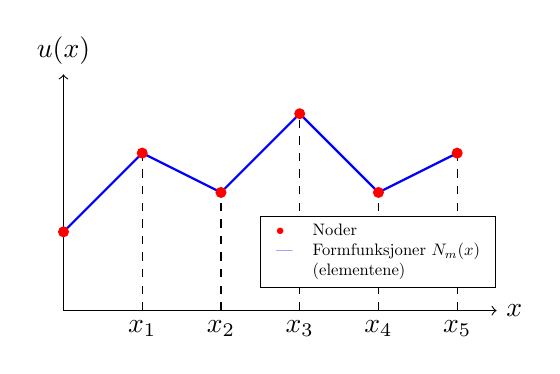
\begin{tikzpicture}
    % Coordinate axes
    \draw[->] (0,0) -- (0,3) node[above] {\(u(x)\)};
    \draw[->] (0,0) -- (5.5,0) node[right] {\(x\)};

    % Solution curve
    \draw[thick, blue] (0,1) -- (1,2) -- (2,1.5) -- (3,2.5) -- (4,1.5) -- (5,2);

    % Vertical lines at nodes with labels
    \draw[dashed] (1,0) node[below] {\(x_1\)} -- (1,2);
    \draw[dashed] (2,0) node[below] {\(x_2\)} -- (2,1.5);
    \draw[dashed] (3,0) node[below] {\(x_3\)} -- (3,2.5);
    \draw[dashed] (4,0) node[below] {\(x_4\)} -- (4,1.5);
    \draw[dashed] (5,0) node[below] {\(x_5\)} -- (5,2);

    % Nodes (intersection points)
    \fill[red] (0,1) circle (2pt);
    \fill[red] (1,2) circle (2pt);
    \fill[red] (2,1.5) circle (2pt);
    \fill[red] (3,2.5) circle (2pt);
    \fill[red] (4,1.5) circle (2pt);
    \fill[red] (5,2) circle (2pt);

    % Add legend
    \node[draw, anchor=north west, scale=0.6,fill=white] at (2.5,1.2) {
      \begin{tabular}{ll}
        \textcolor{red}{$\bullet$} & Noder                     \\
        \textcolor{blue}{---}      & Formfunksjoner \(N_m(x)\) \\
                                   & (elementene)              \\
      \end{tabular}
    };
  \end{tikzpicture}
  \caption{Tilfeldig valgt formfunksjoner \(N_i(x)\) mellom nodene \(x_i\).}
\end{figure}

\begin{equation*}
  \symbf{F} = - \bar{f} \int_0^1 \symbf{N}(x) dx = - \bar{f} \begin{bmatrix}
    0.1 \\ 0.2 \\ 0.2 \\ 0.2 \\ 0.2 \\ 0.1
  \end{bmatrix}
\end{equation*}


\section{Basisfunksjoner}

Basisfunksjoner er byggesteinene i \gls{fem}-metoden.
De er enkle funksjoner som gjør at vi kan representere en komplisert funksjon ved hjelp av enkle byggesteiner.

\subparagraph{\gls{basisfunction}}
En \gls{basisfunction} $\phi_i(x)$ er en lokal funksjon som:
\begin{itemize}
  \item Er null overalt unntatt i nærheten av node \(i\) (lokalt definert).
  \item Har verdien 1 i node \(i\) og 0 i alle andre noder
  \item Til sammen kan bygge opp løsningen vår \(u(x)\) som en sum:
        \[
          u(x) = \sum_{i=1}^n u_i \phi_i(x) = \symbf{u}^T \symbf{\phi}(x)
        \]
  \item \(u_i\) er koeffisientene som bestemmer hvor mye av hver \gls{basisfunction} som skal brukes.
\end{itemize}


\subsection{Stykkvis lineære basisfunksjoner}

La \(u(x)\) være en tilnærming til løsningen av et \gls{pde}, og la \(u(x)\) være gitt ved en lineærkombinasjon av \gls{basisfunction}er:
\[
  u(x) = \sum_{i=1}^6 u_i N_i(x)
\]


\begin{figure}[H]
  \centering
  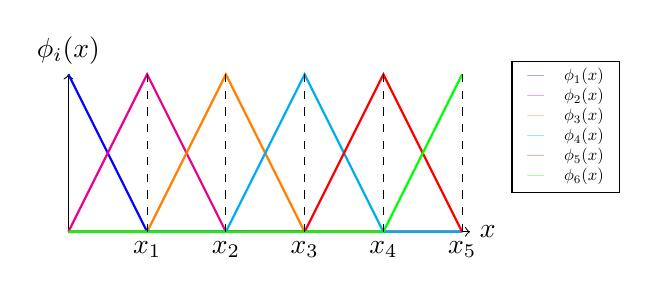
\begin{tikzpicture}
    % Coordinate axes
    \draw[->] (0,0) -- (0,2) node[above] {\(\phi_i(x)\)};
    \draw[->] (0,0) -- (5.1,0) node[right] {\(x\)};

    % Solution curve
    \draw[thick, blue] (0,2) -- (1,0) -- (5,0);
    \draw[thick, magenta] (0,0) -- (1,2) -- (2,0) -- (5,0);
    \draw[thick, orange] (0,0) -- (1,0) -- (2,2) -- (3,0) -- (5,0);
    \draw[thick, cyan] (0,0) -- (2,0) -- (3,2) -- (4,0) -- (5,0);
    \draw[thick, red] (0,0) -- (3,0) -- (4,2) -- (5,0);
    \draw[thick, green] (0,0) -- (4,0) -- (5,2);

    % Vertical lines at nodes with labels
    \draw[dashed] (1,0) node[below] {\(x_1\)} -- (1,2);
    \draw[dashed] (2,0) node[below] {\(x_2\)} -- (2,2);
    \draw[dashed] (3,0) node[below] {\(x_3\)} -- (3,2);
    \draw[dashed] (4,0) node[below] {\(x_4\)} -- (4,2);
    \draw[dashed] (5,0) node[below] {\(x_5\)} -- (5,2);

    % Legend
    \node[draw, anchor=south east, scale=0.6,fill=white] at (7,0.5) {
      \begin{tabular}{ll}
        \textcolor{blue}{---}    & \(\phi_1(x)\) \\
        \textcolor{magenta}{---} & \(\phi_2(x)\) \\
        \textcolor{orange}{---}  & \(\phi_3(x)\) \\
        \textcolor{cyan}{---}    & \(\phi_4(x)\) \\
        \textcolor{red}{---}     & \(\phi_5(x)\) \\
        \textcolor{green}{---}   & \(\phi_6(x)\) \\
      \end{tabular}
    };

  \end{tikzpicture}
  \caption{Piecewise Linear Basis Functions $\phi_i(x)$}
\end{figure}

\section{Svak formulering}
\subsubsection{Sterk formulering av PDE}
Her skriver vi \gls{pde}-en direkte i differensialform. Det betyr at vi forutsetter at løsningen u er glatt nok til at alle deriverte eksisterer. Da har vi:
\[
  \mathcal{L}(u) = f,
\]
samt presise krav på grenseverdier, for eksempel:
\[
  u|_{\partial \Omega} = g \quad \text{eller} \quad \frac{\partial u}{\partial n}\bigg|_{\partial \Omega} = h.
\]

\subsubsection{\gls{weakformulation} av PDE}
Hvis løsningen u ikke er glatt nok, bruker vi en \gls{weakformulation} av problemet.
Her tester vi u med en \gls{testfunction} \(v(x)\) over hele \gls{domain}et:
\[
  \int_\Omega v^{(k)}(x) \, \mathcal{L}(u(x)) \, dx = \int_\Omega v(x) \, f(x) \, dx.
\]
Denne metoden gjør det mulig å finne løsninger i et bredere funksjonsrom.

\gls{testfunction}en er en vilkårlig funksjon som tilfredsstiller randbetingelsene.

\gls{testfunction}en velges ofte til det samme som \gls{basisfunction}en.
\[
  v(x) = \sum_{j=1}^n v_j \phi_j(x) = \symbf{v}^T \symbf{\phi}(x)
\]

\subparagraph{\gls{weakformulation} av Poisson-ligningen}
La oss se på Poisson-ligningen:
\[
  -u''(x) = f(x), \quad x \in (0,1),
\]
med randbetingelser:
\[
  u(0) = \alpha, \quad u(1) = \beta.
\]
Vi kan skrive den svake formuleringen som:
\[
  \int_0^1 v'(x) u'(x) \, dx = \int_0^1 v(x) f(x) \, dx,
\]
Velger \gls{basisfunction}er til å være:
\[
  \phi_i(x) = \begin{cases}
    1 - 2|x - x_i|, & |x - x_i| < 0.5 \\
    0,              & \text{ellers}
  \end{cases}
\]
Med \gls{testfunction}ene \(v(x) = \sum_{j=1}^n v_j \phi_j(x)\).

Da får vi:

\begin{align*}
  \int_0^1 \left( \sum_{j=1}^n v_j \phi_j'(x) \right) \left( \sum_{i=1}^n u_i \phi_i'(x) \right) \, dx
                      & =
  \int_0^1 \left( \sum_{j=1}^n v_j \phi_j(x) \right) f(x) \, dx \\
  \symbf{v}^T \, \int_0^1 \symbf{\phi}' \symbf{\phi}'^T \, dx \, \symbf{u}
                      & =
  \symbf{v}^T \int_0^1 - f(x) \symbf{\phi}  \, dx               \\
  \symbf{v}^T \symbf{K} \symbf{u}
                      & =
  \symbf{v}^T \symbf{F}                                         \\
  \symbf{K} \symbf{u} & = \symbf{F}
\end{align*}

\printglossaries




\subsection{Lecture 8 (28.1.2025)}

\begin{theorem}{Lax-Equivalence-Theorem}{}
    \[
        \text{Consistency} + \text{Stability} \iff \text{Convergence}
    \]
    Holds for linear (time-dependent) problems.
\end{theorem}

PDE:

\begin{align*}
    u_t + u_x  = au, \quad \R \\
    u(x, 0) = f(x) \tag{IC}   \\
    u(0, t) = g(t) \tag{BC}   \\
    u(x,t) =
    \begin{cases}
        e^{at}f(x-t), & x < t \\
        e^{at}g(t-x), & x > t
    \end{cases}
\end{align*}

\paragraph{Scheme:}
\begin{align*}
    U_m^{n+1} = U_m^n - \frac{K}{h}(U_m^n - U_{m-1}^n) + aKU_m^n \\
    \tau_m^n = \frac{1}{2}(K\partial_t^2 u_m^n - h\partial_x^2 u_m^n) + O(K^2 + h^2)
\end{align*}

\[
    \norm{\vec{\tau}^n} \underset{h, K \to 0}{\longrightarrow} 0 \tag{Consistency}
\]

\paragraph{Stencil:}
\begin{figure}[H]
    \centering
    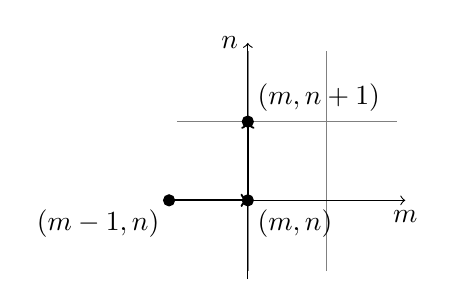
\begin{tikzpicture}
        \draw[step=1cm,gray,very thin] (-0.9,-0.9) grid (1.9,1.9);
        \draw[->] (-1,0) -- (2,0) node[below] {$m$};
        \draw[->] (0,-1) -- (0,2) node[left] {$n$};
        \filldraw[black] (0,0) circle (2pt) node[below right] {$(m,n)$};
        \filldraw[black] (-1,0) circle (2pt) node[below left] {$(m-1,n)$};
        \filldraw[black] (0,1) circle (2pt) node[above right] {$(m,n+1)$};
        \draw[->,thick] (0,0) -- (0,1);
        \draw[->,thick] (-1,0) -- (0,0);
    \end{tikzpicture}
    \caption{Stencil}
    \label{fig:stencil}
\end{figure}

\paragraph{Stability:}
Find \(C\). Define \( S = \frac{K}{h} \).

\[
    U_m^{n+1} = (1 - S + aK)U_m^n + SU_{m-1}^n
\]

\[
    \begin{bmatrix}
        U_1^{n+1} \\
        U_2^{n+1} \\
        \\
        \vdots    \\
        \\
        U_M^{n+1}
    \end{bmatrix}
    =
    \begin{bmatrix}
        1 - S + aK & 0          & 0          & \cdots & 0          \\
        S          & 1 - S + aK & 0          & \cdots & 0          \\
        0          & S          & 1 - S + aK & \cdots & 0          \\
        \vdots     & \vdots     & \vdots     & \ddots & \vdots     \\
        0          & \cdots     & 0          & S      & 1 - S + aK
    \end{bmatrix}
    \begin{bmatrix}
        U_1^n  \\
        U_2^n  \\
        \\
        \vdots \\
        \\
        U_M^n
    \end{bmatrix}
    +
    \begin{bmatrix}
        \overbrace{S g(t_0)}^{U_0^n} \\
        0                            \\
        \vdots                       \\
        0                            \\
        \overbrace{S g(t_n)}^{U_{M+1}^n}
    \end{bmatrix}
\]

\begin{example}{}{}
    \begin{align*}
        u_t = u_{xx} \text{ on } [0,1] \\
        u(x, 0) = f(x)                 \\
        u(1, t) = 0                    \\
        u(0, t) + u_x(0, t) = 0
    \end{align*}
    \paragraph{Scheme}
    let \( r= \frac{K}{h^2} \)
    \[
        U_m^{n+1} = U_m^n + r(U_{m-1}^n - 2U_m^n + U_{m+1}^n)
    \]
    \paragraph{Boundary Conditions}
    \begin{align*}
        U_0^{n+1} = U_0^n + r(U_1^n - 2U_0^n + U_{-1}^n)        \\
        U_0^n + \frac{1}{2h}(U_1^n - U_{-1}^n) = 0              \\
        U_{-1}^n = U_1^n + 2hU_0^n                              \\
        U_0^{n+1} = U_0^n + r(U_1^n - 2U_0^n + U_1^n + 2hU_0^n) \\
        U_0^{n+1} = U_0^n + r(2U_1^n - 4U_0^n)                  \\
        U_0^{n+1} = U_0^n + 2rU_1^n - 4rU_0^n                   \\
        U_0^{n+1} = (1 - 2r(1 - h))U_0^n + 2rU_1^n
    \end{align*}
    Let \( \vec{U}^n = \begin{bmatrix} U_0^n \\ U_1^n \\ \vdots \\ U_M^n \end{bmatrix} \) where \( U_M^n = 0 \).

    \[
        C = \begin{bmatrix}
            1 - 2r(1 - h) & 2r     & 0      & \cdots & 0      \\
            r             & 1 - 2r & r      & \cdots & 0      \\
            0             & r      & 1 - 2r & \cdots & 0      \\
            \vdots        & \vdots & \vdots & \ddots & \vdots \\
            0             & \cdots & 0      & r      & 1 - 2r
        \end{bmatrix}
    \]

    Need to find \( r \leq \frac{1}{2} \) for \(m = 1, 2, \ldots, M-1\) to ensure stability.
    For \( m = 0 \) we need:
    \begin{align*}
        \abs{1 - 2r(1 - h)} + \abs{2r} \leq 1 + \mu K \\
        \abs{1 - 2r(1 - h)} + 2r \leq \abs{1 - 2r} + 2rh + \abs{2r} = 1 + 2rh = 1 + \underbrace{\frac{2}{h}}_{\mu}K
    \end{align*}
    Stable for a given \( h \) but not when \( h \to 0 \).
    \begin{align*}
        K \tau_0^n =                              & u(0, t_n + h) - u(0, t_n) + 2r(1 - h)u(0, t_n) - 2ru(h, t_n)                                                                                                                                            \\                                                                                                                                                                                                                    \\
        =            u_0^n + K \partial_t u_0^n + & \frac{1}{2}K^2 \partial_t^2 u_0^n + \ldots - u_0^n                                                                                                                                                      \\
        +                                         & 2\frac{K}{h^2}(1 - h)u_0^n - 2\frac{K}{h^2}(u_0^n + h \partial_x u_0^n + \frac{1}{2}h^2 \partial_x^2 u_0^n + \frac{1}{6}h^3 \partial_x^3 u_0^n + \frac{1}{24}h^4 \partial_x^4 u_0^n + \ldots)           \\
                                                  & = \frac{K}{h^2}\left[-h(u_0^n + \partial_x u_0^n)\right] + K \left[\partial_t u_0^n - \partial_x^2 u_0^n\right] - \frac{1}{3}Kh\partial_x^3 u_0^n + \ldots + \frac{1}{2}K^2 \partial_t^2 u_0^n + \ldots \\
        K \tau_0^n                                & = -\frac{1}{3}Kh\partial_x^3 u_0^n + \ldots + \frac{1}{2}K^2 \partial_t^2 u_0^n + \ldots \tag{Consistency}
    \end{align*}
\end{example}

\subsection*{Alternative stability analysis: Von Neumann analysis}
Von Neumann analysis is a method for analyzing the stability of finite difference schemes for linear partial differential equations.
The method is based on the Fourier analysis of the numerical solution.

\begin{theorem}{Parseval's equality}{}
    \[
        \sum_{l=-\infty}^{\infty} \abs{C_l}^2 = \frac{1}{2\pi} \int_0^{2\pi} \abs{f(x)}^2 \dd{x}
    \]
\end{theorem}

\begin{example}{}{}
    \begin{align*}
        u_t = u_{xx} \text{ on } [0,1] \\
        u(x, 0) = f(x)                 \\
    \end{align*}
    Make a periodic extension of \(f\), s.t. \(f(x) = f(x-1)\).
    Assue that \(u(x-1, t) = u(x, t)\) and \(u(1, t) = u(0, t)\).
    Write \(f(x)\) as a complex Fourier series:
    \begin{align*}
        f(x) & = \sum_{k=-\infty}^{\infty} C_l e^{i \beta_l x}, \quad \beta_l = 2\pi l, \quad l \in \Z \\
        C_l  & = \int_0^1 f(x) e^{-i \beta_l x} \dd{x}
    \end{align*}

    Seperation of variables:
    \[
        u_l(x, t) = e^{-\beta_l^2 t} e^{i \beta_l x}
    \]
    Plug in the (IC):
    \[
        u(x, t) = \sum_{l=-\infty}^{\infty} C_l e^{-\beta_l^2 t} e^{i \beta_l x}
    \]
    \subparagraph{Idea}
    Given a scheme for \(u_t = u_{xx}\), we can write:
    \[
        U_m^{n+1} = U_m^n + r(U_{m-1}^n - 2U_m^n + U_{m+1}^n), \quad r = \frac{k}{h^2}
    \]

    Search for a solution of the form:
    \[
        U_m^n = \psi^n e^{i \beta x_m}
    \]
    A scheme is \textit{Von Neumann stable} if:
    \[
        \abs{\psi} < 1 + \mu k, \quad \mu \geq 0
    \]

    In our example:
    \begin{align*}
        \psi^{n+1} e^{i \beta x_m} & = \psi^n e^{i \beta x_m} + r\psi^n\left(e^{i \beta x_{m+1}} - 2e^{i \beta x_m} + e^{i \beta x_{m-1}}\right) \\
                                   & = \psi^n e^{i \beta x_m} (1 + r(e^{i \beta h} - 2 + e^{-i \beta h}))                                        \\
        \psi                       & = 1 + r(e^{i \beta h} - 2 + e^{-i \beta h})                                                                 \\
                                   & = 1 + r(2\cos(\beta h) - 2)                                                                                     \\
                                      & = 1 + 4r\sin^2\left(\frac{\beta h}{2}\right)                                                                    \\
        \abs{\psi}                 & = \abs{1 + 4r\sin^2\left(\frac{\beta h}{2}\right)} \leq 1 \iff r \leq \frac{1}{2}, \forall \beta \text{ and } \mu = 0
    \end{align*}
\end{example}

\section{Forelesninger}

\subsection{Mandag \date{3. februar 2025}}

\paragraph{Von Neumann Stability Analysis}

\begin{itemize}
  \item Let \( U_m^n = \xi^n e^{i\beta m} \). Insert this into Difference Equation (DE).
  \item The method is Von Neumann Stable if \( \abs{\xi} \leq 1 + \mu K \) for all \( \beta \).
  \item Von Neumann stability is sufficient and necessary for pure IVP problems (Cauchy problems).
\end{itemize}
\begin{figure}[H]
  \centering
  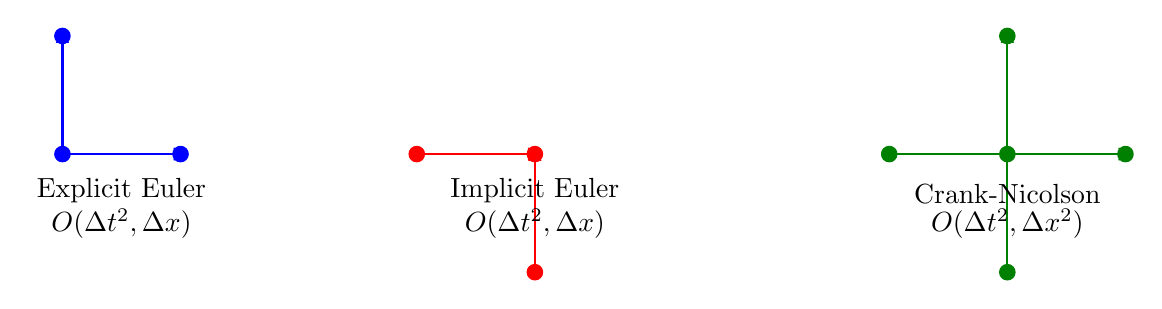
\begin{tikzpicture}[scale=1.5]
    % Explicit Euler (Forward)
    \begin{scope}[xshift=0cm]
      \fill[blue] (0,0) circle (2pt);
      \fill[blue] (0,1) circle (2pt);
      \fill[blue] (1,0) circle (2pt);
      \draw[->,thick,blue] (0,0) -- (1,0);
      \draw[->,thick,blue] (0,0) -- (0,1);
      \node[above] at (0.5,-0.5) {Explicit Euler};
      \node[above] at (0.5,-0.8) {\(O(\Delta t^2, \Delta x)\)};
    \end{scope}

    % Implicit Euler (Backward)
    \begin{scope}[xshift=4cm]
      \fill[red] (0,0) circle (2pt);
      \fill[red] (-1,0) circle (2pt);
      \fill[red] (0,-1) circle (2pt);
      \draw[->,thick,red] (-1,0) -- (0,0);
      \draw[->,thick,red] (0,-1) -- (0,0);
      \node[above] at (0,-0.5) {Implicit Euler};
      \node[above] at (0,-0.8) {\(O(\Delta t^2, \Delta x)\)};
    \end{scope}

    % Crank-Nicolson
    \begin{scope}[xshift=8cm]
      \fill[green!50!black] (0,0) circle (2pt);
      \fill[green!50!black] (1,0) circle (2pt);
      \fill[green!50!black] (-1,0) circle (2pt);
      \fill[green!50!black] (0,1) circle (2pt);
      \fill[green!50!black] (0,-1) circle (2pt);
      \draw[->,thick,green!50!black] (-1,0) -- (1,0);
      \draw[->,thick,green!50!black] (0,-1) -- (0,1);
      \node[above] at (0,-0.5) {Crank-Nicolson};
      \node[above] at (0,-0.8) {\(O(\Delta t^2, \Delta x^2)\)};
    \end{scope}
  \end{tikzpicture}
  \caption{Stencils for different numerical schemes}
  \label{fig:stencils}
\end{figure}



\begin{example}{Heat equation}{}
  \[
    u_t = u_{xx}, \quad 0 \leq x \leq 1, \quad 0 \leq t \leq 0.5
  \]
  \[
    \begin{cases}
      u(x, 0) = \sin(\pi x) \\
      u(0, t) = u(1, t) = 0
    \end{cases}
  \]
  \[
    u(x, t) = \sin(\pi x) e^{-\pi^2 t}
  \]

  \subparagraph{Finite Difference Scheme}
  \[
    \frac{1}{2k}\left( U_m^{n+1} - U_m^{n-1} \right) = \frac{1}{h^2}\left( U_{m-1}^n - 2U_m^n + U_{m+1}^n \right)
  \]

  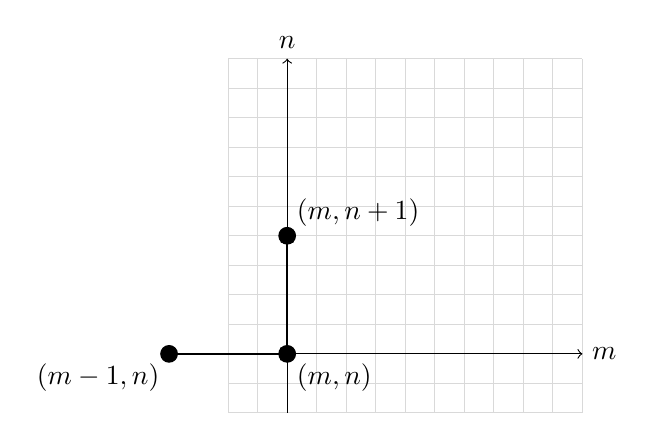
\begin{tikzpicture}[scale=1.5]
    % Grid
    \draw[step=0.25cm,gray!30] (-0.5,-0.5) grid (2.5,2.5);
    \draw[->] (-0.5,0) -- (2.5,0) node[right] {$m$};
    \draw[->] (0,-0.5) -- (0,2.5) node[above] {$n$};
    % Points
    \filldraw[black] (0,0) circle (2pt) node[below right] {$(m,n)$};
    \filldraw[black] (-1,0) circle (2pt) node[below left] {$(m-1,n)$};
    \filldraw[black] (0,1) circle (2pt) node[above right] {$(m,n+1)$};
    % Arrows
    \draw[->,thick] (0,0) -- (0,1);
    \draw[->,thick] (-1,0) -- (0,0);

  \end{tikzpicture}


  \subparagraph{Fourier Stability Analysis}

  \begin{align*}
    U_m^{n+1}
     & =
    2r\left( U_{m-1}^n - U_m^n + U_{m+1}^n \right) + U_m^{n-1}               \\
    \xi^{n+1} e^{i\beta x_m}
     & =
    2r\xi^n
    \left[
      e^{i\beta x_m - h} - 2e^{i\beta x_m} + e^{i\beta x_m + h}
      \right]
    + \xi^{n-1} e^{i\beta x_m}                                               \\
    \xi^2
     & =
    2r\left[ e^{-i\beta h} - 2 + e^{i\beta h} \right]\xi + 1                 \\
    \xi^2
     & =
    2r \left[ 2\cos(\beta h) - 2 \right]\xi+ 1                               \\
    \xi^2 + 8r\sin^2 \frac{\beta h}{2}\xi - 1
     & =
    0 \quad  \implies \quad \xi_\pm
    =
    -4r\sin^2 \frac{\beta h}{2} \pm \sqrt{16r^2\sin^4 \frac{\beta h}{2} + 1} \\
    \xi_- \leq - 1
    \quad
    \abs{\xi_-} \leq 1
  \end{align*}

  \textbf{Conclusion:} The scheme is unconditionally unstable.

  But we can stabilize the scheme by introducing a damping term (Du Fort-Frankel scheme):
  Replace \( U_m^n \leftarrow \frac{1}{2}(U_m^{n+1} + U_m^{n-1}) \) in the scheme.

  \begin{align*}
    \frac{1}{2k}\left( U_m^{n+1} - U_m^{n-1} \right)
     & =
    \frac{1}{h^2}\left( U_{m-1}^n + U_{m+1}^n\right) - \frac{1}{h^2}\left( U_m^{n+1} + U_m^{n-1} \right) \\
    (1 + 2r)U_m^{n+1}
     & =
    2r\left( U_{m-1}^n + U_{m+1}^n \right) + (1 - 2r)U_m^{n-1}                                           \\
    (1 + 2r)\xi^2 - 4r \cos \beta h \xi - (1 - 2r)
     & = 0                                                                                               \\
    \xi_\pm
     & = \frac{1}{1 + 2r} \left[ 2r\cos \beta h \pm \sqrt{4r^2\cos^2 \beta h + (1 - 2r)(1 + 2r)} \right] \\
    \xi_\pm
     & = \frac{1}{1 + 2r} \left[ 2r\cos \beta h \pm \sqrt{1 - 4r^2 \sin^2 {bh}} \right]                  \\
    \abs{\xi_\pm}^2 = \frac{2r - 1}{2r + 1} < 1 \quad \text{for all } r                                  \\
  \end{align*}

  \textbf{Conclusion:} The method scheme is unconditionally stable, for all \( r \).

  Now we know that the scheme has stability for all \( r \), it might still not converge because we also need consistency.

  \subparagraph{Consistency}
  \begin{align*}
    \tau_m^n
     & =
     & \frac{1}{2k}\left( u_m^{n+1} - u_m^{n-1} \right)                                                 \\
     & - \frac{1}{h^2}\left( u_{m-1}^n - u_{m+1}^n \right)                                              \\
     & + \frac{1}{h^2}\left( u_m^{n+1} - u_m^{n-1} \right)                                              \\
     & =
     & \frac{1}{2k}\left[ 2k u_t + 2k^3 \frac{1}{3!}u_{tt} + \ldots \right]                             \\
     & -\frac{1}{h^2}\left[ 2u + 2h^2 \frac{1}{2!}u_{xx} + 2h^4 \frac{1}{4!}u_{xxxx} + \ldots \right]   \\
     & + \frac{1}{h^2}\left[ 2 u + 2k^2 \frac{1}{2!}u_{tt} + 2k^4 \frac{1}{4!}u_{tttt} + \ldots \right] \\
     & =
    u_t - u_xx
    + \frac{k^2}{h^2}u_{tt} + \frac{k^2}{3!}u_{tt}
    + \frac{h^2}{12}u_{xxxx} + \frac{k^4}{12h^2}u_{tttt}
    + \ldots
  \end{align*}
  The method is consistent only if the truncation error goes to zero as \( h, k \to 0 \).

  Here the method is consistent when \(\frac{k}{h} \underset{h,k \to 0}{\longrightarrow} 0\).

  \textbf{Conclusion:} The method is conditionally consistent.

  \textbf{Conclusion:} The method is conditionally stable and consistent for all \( r \) and \( \frac{k}{h} \underset{h,k \to 0}{\longrightarrow} 0 \) and therefore convergent.

\end{example}

\paragraph{Domain of dependence}

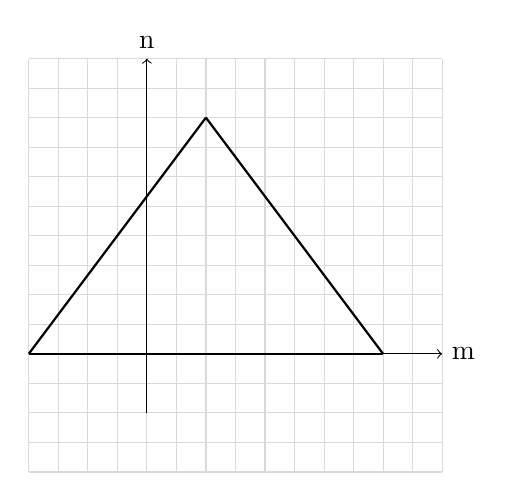
\begin{tikzpicture}[scale=1.5]
  % Grid
  \draw[step=0.25cm,gray!30] (-1,-1) grid (2.5,2.5);
  \draw[->] (-1,0) -- (2.5,0) node[right] {m};
  \draw[->] (0,-0.5) -- (0,2.5) node[above] {n};

  % Triangle
  \draw[-,thick] (-1,0) -- (0.5,2);
  \draw[-,thick] (-1,0) -- (2,0);
  \draw[-,thick] (2,0) -- (0.5,2);

\end{tikzpicture}


\subsection{Tirsdag \date{4. februar 2025}}

\paragraph{Hyperbolic PDEs}

\begin{align*}
  a u_{xx} + 2bu_{xy} + c u_{yy} = f(x,y, u, u_x, u_y) \tag{1} \\
  \begin{cases}
    b^2 - ac > 0 & \text{Hyperbolic} \\
    b^2 - ac = 0 & \text{Parabolic}  \\
    b^2 - ac < 0 & \text{Elliptic}
  \end{cases}                             \\
\end{align*}\label{eq:hb1}

\begin{example}{Wave equation}{}
  \begin{align*}
    u_{tt} & = c^2 u_{xx}                                                                                   \\
    u(x,0) & = f(x), \quad u_t(x,0) = g(x)                                                                  \\
    u(x,t) & = \frac{1}{2}\left[ f(x - ct) + f(x + ct) \right] + \frac{1}{2c} \int_{x-ct}^{x+ct} g(s) \, ds
  \end{align*}
\end{example}

\subparagraph{D'Alembert's principle}
\begin{figure}[H]
  \centering
  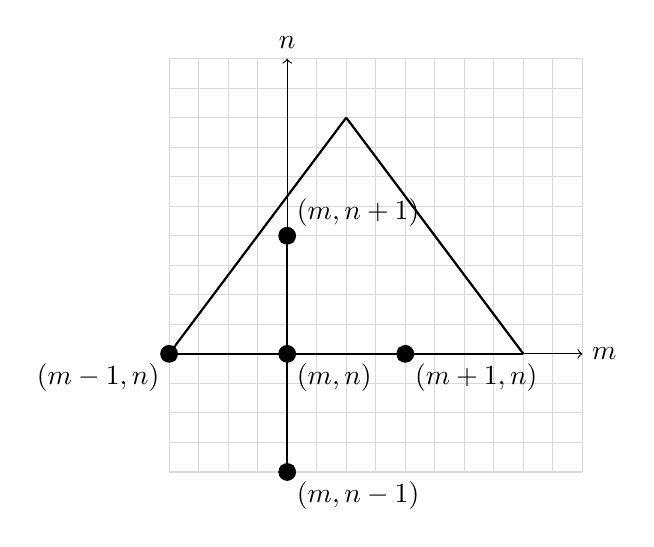
\begin{tikzpicture}[scale=1.5]
    % Grid
    \draw[step=0.25cm,gray!30] (-1,-1) grid (2.5,2.5);
    \draw[->] (-1,0) -- (2.5,0) node[right] {$m$};
    \draw[->] (0,-0.5) -- (0,2.5) node[above] {$n$};

    % Triangle
    \draw[-,thick] (-1,0) -- (0.5,2);
    \draw[-,thick] (-1,0) -- (2,0);
    \draw[-,thick] (2,0) -- (0.5,2);

    % Points
    \filldraw[black] (0,0) circle (2pt) node[below right] {$(m,n)$};
    \filldraw[black] (-1,0) circle (2pt) node[below left] {$(m-1,n)$};
    \filldraw[black] (0,1) circle (2pt) node[above right] {$(m,n+1)$};
    \filldraw[black] (1,0) circle (2pt) node[below right] {$(m+1,n)$};
    \filldraw[black] (0,-1) circle (2pt) node[below right] {$(m,n-1)$};

    % Arrows
    \draw[->,thick] (0,0) -- (0,1);
    \draw[->,thick] (0,0) -- (1,0);
    \draw[->,thick] (0,0) -- (-1,0);
    \draw[->,thick] (0,0) -- (0,-1);

  \end{tikzpicture}
  \caption{Stencils for the wave equation}
  \label{fig:wave-stencils}
\end{figure}

\begin{align*}
  Lu          & = \partial_t^2 u - c^2 \partial_x^2 u = (\partial_t - c \partial_x)(\partial_t + c \partial_x)u = 0 \\
  u_t + c u_x & = v                                                                                                 \\
  v_t - c v_x & = 0
\end{align*}

\subparagraph{1st order equations}
\begin{itemize}
  \item Density: \(u\)
  \item Non-conservative: \[ u_t + a(x,t,u)u_x = b(x,t,u) \tag{2} \]\label{eq:hb2}
  \item Transport equation: \(u_t + au_x = 0\) where \(a\) is a constant.
        \[
          \dd{t} \int_{x_1}^{x_2} u(x,t) \, dx = \int_{x_1}^{x_2} u_t(x,t) \, dx = -\int_{x_1}^{x_2} (f(u))_x \, dx = f(u(x_1,t)) - f(u(x_2,t))
        \]
  \item Conservation laws: \(u_t + (f(u))_x = 0\)
\end{itemize}

\subparagraph{1st order system}
\begin{itemize}
  \item Non-conservative: \[\symbf{u_t} + A(\symbf{u}_x) = \symbf{b}\tag{3}\]\label{eq:hb3}
  \item Conservative: \[\symbf{u_t} + (\symbf{f}(\symbf{u}))_x = 0\]
        This is hyperbolic if \(A\) is diagonalizable with real eigenvalues.
        \[
          A = PDP^{-1} \quad \text{where} \quad D = \text{diag}(\lambda_1, \ldots, \lambda_n)
        \]
        Equivalently, if the Jacobian matrix of \(\symbf{f}\) is diagonalizable with real eigenvalues.

        For linear problems (Hyperbolic PDEs),\eqref{eq:hb1} can always be written as \eqref{eq:hb3}.
        \eqref{eq:hb3} can always be decoupled into a set of \eqref{eq:hb2} equations.
\end{itemize}
\paragraph{Method of Characteristics}
Let \(u_t + a(x,t,u)u_x = b(x,t,u)\) be a non-conservative hyperbolic PDE. Furthermore let \(v(t) = u(x(t), t)\) where \(x(t)\) is a characteristic curve. Then
\[
  \dot{v} = u_x \dot{x} + u_t = u_t + a(x,t,u)u_x = b(x(t), t, u(x(t), t)=v(t))
\]
Let \(\dot{x} = a(x,t,u)\) (characteristic equation) and \(\dot{v} = b(x(t), t, v(t))\) (System of ODEs).
Initial values: \(\begin{cases} x(t_0) = x_0 \\ v(t_0) = u(x_0, t_0) \end{cases}\) is known for all \((t_0, x_0)\) on the initial curve.

\begin{align*}
  x(t) & = \mathcal{X}(t; t_0, x_0), \quad x_0 = x(t_0) = \mathcal{X}^{-1}(x, t)               \\
  v(t) & = \mathcal{V}(t; x_0, t_0, u_0), \quad u(x,t) = \mathcal{V}(t, \mathcal{X}^{-1}(x,t))
\end{align*}

\begin{example}{\(u_t + a u_x = b\) where \(a, b\) can be functions of \(x, t, u\)}{}
  \begin{align*}
    u_t + a(x,t,u)u_x & = b(x,t,u)                                                                                                          \\
    u(x,0)            & = u_0(x)   \quad \Sigma \text{ is the initial curve}                                                                \\
    \dot{x(t)}        & = a, \quad x(0) = x_0 \implies x(t) = x_0 + at \implies x_0 = x - at \implies u(x_0, 0) = u_0(x_0) \text{ is known} \\
    \dot{v(t)}        & = b
  \end{align*}

  % FYLL FRA BILDER PÅ TLF!

\end{example}


\subparagraph{Finite Difference Scheme}
\[
  \frac{1}{k^2}\left( U_m^{n+1} - 2U_m^n + U_m^{n-1} \right) = \frac{1}{h^2}\left( U_{m-1}^n - 2U_m^n + U_{m+1}^n \right)
\]

\subparagraph{Von Neumann Stability Analysis}
\begin{align*}
  U_m^n         & = \xi^n e^{i\beta m}                                                    \\
  \xi^2         & = \frac{1}{r^2} - 2 + \frac{1}{r^2} = 2\left( \frac{1}{r^2} - 1 \right) \\
  \xi_\pm       & = \pm \sqrt{2\left( \frac{1}{r^2} - 1 \right)}                          \\
  \abs{\xi_\pm} & \leq 1 \quad \text{if} \quad r \geq 1
\end{align*}

\textbf{Conclusion:} The method is conditionally stable.

\subparagraph{Consistency}
\[
  \tau_m^n = \frac{1}{k^2}\left( u_t - u_{xx} \right) + O(k^2, h^2)
\]

\textbf{Conclusion:} The method is consistent.

\textbf{Conclusion:} The method is conditionally stable and consistent and therefore convergent.


\begin{example}{}{}

  \[
    u_t + e^{-x}u_x = 0, \quad u(x,0) = u_0(x)
  \]

  \textbf{Method of Characteristics:}
  \begin{align*}
    \dot{x} & = e^{-x}, \quad x(0) = x_0             \\
    \dot{v} & = 0, \quad v(0) = u(x_0, 0) = u_0(x_0)
  \end{align*}
  \begin{align*}
    \frac{dx}{dt} = e^{-x} & \implies \int_{x_0}^x e^x \, dx = \int_0^t \, dt \implies e^x - e^{x_0} = t \implies x_0 = \ln(e^x - t) \\
    \frac{dv}{dt} = 0      & \implies v = u_0(x_0) = u_0(\ln(e^x - t))
  \end{align*}

\end{example}


\subsection{Onsdag \date{10. februar 2025}}

\paragraph{What about systems?}

\begin{align*}
  \symbf{u_t} + A(\symbf{u}_x)                           & = \symbf{0} \\
  \symbf{u_t} + P\Lambda P^{-1}(\symbf{u}_x)             & = \symbf{0} \\
  P^{-1}\symbf{u_t} + \Lambda P^{-1}\Lambda(symbf{u}_x) & = \symbf{0} \\
  \symbf{v_t} + \Lambda \symbf{v}_x                      & = \symbf{0}
\end{align*}

Hyperbolic if \(A\) is diagonalizable with real eigenvalues: \(A = P\Lambda P^{-1}\) where \(\Lambda = \text{diag}(\lambda_1, \ldots, \lambda_n)\).

\begin{example}{}{}
  \begin{align*}
    \symbf{v_{i,t} + \lambda_i v_{i,x} = 0}                                  \\
    \symbf{u}_t +
    \begin{bmatrix}
      a & b \\
      c & d
    \end{bmatrix}
    \symbf{u}_x = \symbf{0} \quad \text{where} \quad x\in [0,1], \quad t \geq 0 \\
    \symbf{u}(x,0) = \symbf{f}(x) \quad \text{is the initial curve}
  \end{align*}

  Then the eigenvalues are \(\lambda_{1,2} = a \pm b\) with eigenvectors
  \[
    P = \begin{bmatrix}
      1 & 1  \\
      1 & -1
    \end{bmatrix}
  \]
  and
  \[
    \symbf{v} = P^{-1}\symbf{u} \implies \symbf{u} = P\symbf{v}
  \]

  then we get the system

  \begin{align*}
    \symbf{v}_{1,t} + (a + b)\symbf{v}_{1,x} & = 0 \\
    \symbf{v}_{2,t} + (a - b)\symbf{v}_{2,x} & = 0
  \end{align*}

  assume that \(a > 0\), with the BCs
  \[
    x=0 \quad \text{inflow if } \lambda > 0 \quad \vee quad x = 1 \quad \text{outflow if } \lambda < 0
  \]

  \subparagraph{Case 1}
  \[
    a > b \quad \text{and} \quad \lambda_1, \lambda_2 > 0
  \]



\end{example}


\paragraph{Scheming}
\[
  \symbf{u}_t + a \symbf{u}_x = 0 , \quad b \in \R \quad \symbf{u}(x,0) = \symbf{f}(x)
\]

%draw Grid
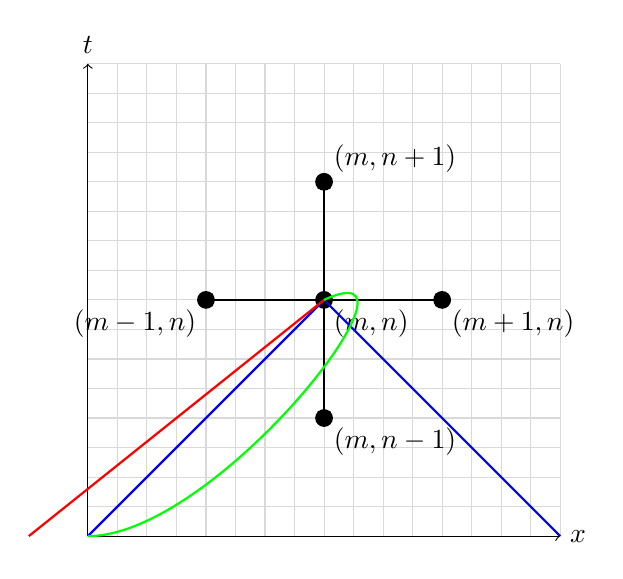
\begin{tikzpicture}[scale=1.5]
  % Grid
  \draw[step=0.25cm,gray!30] (-1,-1) grid (3,3);
  \draw[->] (-1,-1) -- (3,-1) node[right] {$x$};
  \draw[->] (-1,-1) -- (-1,3) node[above] {$t$};

  % Points
  \filldraw[black] (1,1) circle (2pt) node[below right] {$(m,n)$};
  \filldraw[black] (0,1) circle (2pt) node[below left] {$(m-1,n)$};
  \filldraw[black] (1,2) circle (2pt) node[above right] {$(m,n+1)$};
  \filldraw[black] (2,1) circle (2pt) node[below right] {$(m+1,n)$};
  \filldraw[black] (1,0) circle (2pt) node[below right] {$(m,n-1)$};

  % Stencils
  \draw[->,thick] (1,1) -- (1,2);
  \draw[->,thick] (1,1) -- (2,1);
  \draw[->,thick] (1,1) -- (0,1);
  \draw[->,thick] (1,1) -- (1,0);

  % Stencil 2 (Orange)
  \draw[-,thick,blue] (-1,-1) -- (1,1);
  \draw[-,thick,blue] (3,-1) -- (1,1);

  % Stencil 3 (red, outside)
  \draw[-,thick,red] (-1.5,-1) -- (1,1);

  % Stencil 4 (green, curved inside)
  \draw[-,thick,green] (-1,-1) to [out=0,in=25] (1,1);



\end{tikzpicture}

\subparagraph{Central Time, Central Space}
\[
  \frac{1}{k}\left( U_m^{n+1} - U_m^{n-1} \right) = \frac{1}{h}\left( U_{m+1}^n - U_{m-1}^n \right)
\]

\subparagraph{Forward Time, Central Space}
\[
  \frac{1}{k}\left( U_m^{n+1} - U_m^n \right) = \frac{1}{h}\left( U_{m+1}^n - U_{m-1}^n \right)
\]

´
Then
\[
  U_m^{n+1} = \beta_{-1} U_{m-1}^n + \beta_0 U_m^n + \beta_1 U_{m+1}^n
\]

Assume that \(\beta_{-1} \neq 0\) and \(\beta_1 \neq 0\), then the method is unconditionally unstable.

\begin{align*}
  T = k n                                                     \\
  x_{m-n} = \mathcal{X} - \dfrac{T}{k}h = \mathcal{X} - \mu T \\
  x_{m+n} = \mathcal{X} + \dfrac{T}{k}h = \mathcal{X} + \mu T
\end{align*}

Interval of dependence: \(\left[ \mathcal{X} - \mu T, \mathcal{X} + \mu T \right]\)

Domain of dependence: Triangle of this and \((X,T)\).

\subparagraph{Characteristics}

\begin{align*}
  x = x_0 + at \implies x_0 = x - at \quad \text{goes through} \quad (\mathcal{X}, T) \\
  x_0 = \mathcal{X} - \mu T \quad \text{CFL condition} \\
  \text{We need} \quad x_0 = \mathcal{X} - \mu T \in [X - \mu T, X + \mu T] \\
  \abs{a} \frac{k}{h} \leq 1 \quad \text{CFL condition}
\end{align*}

\subparagraph{Forward Time, Backward Space}
\[
  \frac{1}{k}\left( U_m^{n+1} - U_m^n \right) = a \frac{1}{h}\left( U_m^n - U_{m-1}^n \right)
\]

Let \(p = a \frac{k}{h}\), then

\[
  U_m^{n+1} = U_m^n + p(U_{m-1}^n - U_m^n)
\]

\subparagraph{Von Neumann Stability Analysis}
\[
  U_m^n = \xi^n e^{i\beta m} \quad \beta \in \R
\]

Stable if there is a \(\mu> 0\) such that \(\abs{\xi} \leq 1 + \mu k \).

For the FTBS scheme, we get

\begin{align*}
  \xi^{n+1} e^{i\beta m} & = \xi^n e^{i\beta m} + p\xi^n\left( e^{i\beta m} - e^{i\beta (m-1)} \right) \\
  \xi                   & = 1 - p(1 - e^{-i\beta h}) = (1 - p) + pe^{-i\beta h}                            \\
\end{align*}

Here we can see that \(\abs{\xi} \) is just a circle in the complex plane with radius \(p\) and center \((1-p)\).

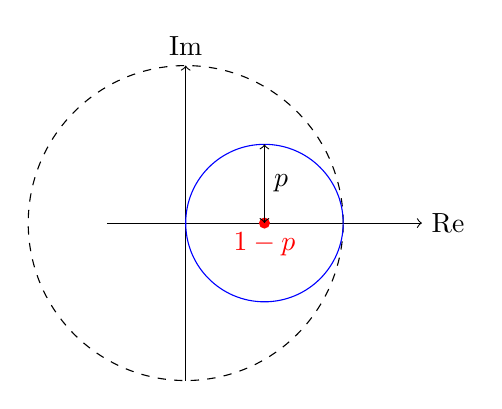
\begin{tikzpicture}[scale=2]
  % Parameters
  \def\p{0.5}

  % Axes
  \draw[->] (-0.5,0) -- (1.5,0) node[right] {Re};
  \draw[->] (0,-1) -- (0,1) node[above] {Im};
  
  % Unit circle
  \draw[dashed] (0,0) circle (1);
  
  % Circle representing xi
  \draw[blue] (1-\p,0) circle (\p);
  
  % Center point
  \fill[red] (1-\p,0) circle (1pt) node[below] {$1-p$};
  
  % Radius label
  \draw[<->] (1-\p,0) -- ++(0,\p) node[midway,right] {$p$};
\end{tikzpicture}

So the scheme is stable if \(\abs{\xi} \leq 1 \) if \(0 < p \leq 1\) or \(0 < a \frac{k}{h} \leq 1\).

What happens if we have \(a < 0\)? In this case the condition \(\abs{\xi} \leq 1 \) for all \( \beta \) is not satisfied.

\subparagraph{Forward Time, Central Space}

\[
  U_m^{n+1} = U_m^n - \frac{p}{2}\left( U_{m+1}^n - U_{m-1}^n \right)
\]

Then we get the stability condition:

\begin{align*}
  \xi & = 1 - \frac{p}{2}\left( e^{i\beta h} - e^{-i\beta h} \right) = 1 - p\sin(\beta h) \\
  \abs{\xi} & = \sqrt{(1 - p\sin^2(\beta h))} = 1 - p\sin(\beta h) \leq 1
\end{align*}





\end{document}